\chapter{Design and Implementation - Import}
\label{chapter:Design and Implementation - Import}



In the next two chapters, we will discuss about the steps taken to import our dataset into a fully tuned HBase cluster deployed on top of Triton. We will go through a basic version of importing data to the most fine-grain solution we managed to get, but before going into details, let us depict the work-flow taken, doing your reading more satisfactory and easier.


\bigskip
\begin{figure}[htb]
\centering
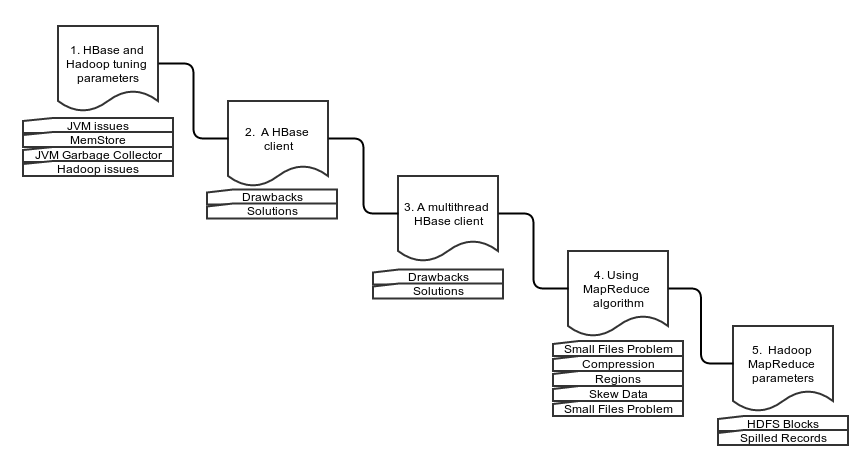
\includegraphics[width=1\textwidth]{./images/approaches.png}
\caption{Import research workflow.} \label{fig:approaches}
\end{figure}




\section{HBase cluster at a glance}

We use a 5 nodes HBase cluster by default: 1 Master server and 4 Region Servers. Default parameters are described below. Whether there is a change in the number of nodes or any parameters, we will state it in its corresponding section.
\par
As we exposed in chapter 4, we use HBase in combination with HDFS as our distributed filesystem. Hence, we deploy a DataNode in the same node where HBase Master is and a DataNode along with each Region Server. Besides it, if the task requires Hadoop MapReduce, we turn it on, starting a JobTracker where the NameNode is and as many TaskTrackers as DataNodes there are in the cluster.

\section{HBase: tunning parameters for a write-heavy cluster}

In this section, we will explain how we have optimized our HBase cluster to meet our needs, which could be summarized into "excel in importing data" operations.
\par
HBase is highly configurable when it comes to data-writing with plenty modifiable parameters. In the following lines we specify which ones, why and how we have modified them. They are Java Virtual Machine parameters, MemStore parameters and a few Hadoop parameters.

\begin{enumerate}

\item \textbf{JVM related parameters}:
\bigskip

- \textit{HBASE\_HEAPSIZE}: 
\par
The maximum amount of heap to allocate expressed in MB. We have increased this parameter from 1000 to 2000 as HBase is a RAM consumer. The more RAM, the better the performance.
\par
- \textit{HBASE\_OPTS}:
\par
We have enabled Java's garbage collector logs as a way to help us to discover how to improve performance by tuning JVM flags and looking for long and short pauses. 
\par
Following Todd Lipcon blog articles "Avoiding Full GCs in Apache HBase with MemStore-Local Allocation Buffers: Part 1, 2 and 3" \footnote{http://blog.cloudera.com/blog/2011/02/avoiding-full-gcs-in-hbase-with-memstore-local-allocation-buffers-part-1/}, we have turned on the \textit{Parallel New} collector for the young generation (\textit{-XX:+UseParNewGC}) and the \textit{Concurrent Mark-Sweep} collector for the old generation (\textit{-XX:+UseConcMarkSweepGC}). The Parallel New collector is a "stop-the-world copying collector" but since the young generation is small and it uses many threads, the collector finishes its work very quickly and no stops are appreciate.
\par
The Concurrent-Mark-Sweep collector (CMS) is responsible for cleaning dead objects in the old generation. It is also a "stop-the-world collector". The problem comes out when CMS fails and minute pauses appear in logs. CMS has two failure modes:
\begin{enumerate}
\item \textbf{Concurrent Mode Failure}: To avoid this mode, we need the garbage collector to start its work earlier in order to avoid getting overrun with new allocations. Setting \textit{-XX:CMSInitationOccupancyFraction} flag to 70 turns out to help us.
\item \textbf{Promotion Failure Mode due to fragmentation}: This happens when there is not enough contiguous free space in the old-generation to allocate objects. This is termed memory fragmentation. When this occurs, the copying collector is called owing to its ability to compact all objects and free up space. To address this issue and avoid the stop produced by the copying collector, we use MemStore-Local Allocation Buffer (MSLAB) \footnote{MSLAB articles for a deeper background \cite{ApacheHBaseMSLAB} \cite{MSLAB})}, a new Todd's experimental facility.  \textit{Hbase.hregion.memstore.mslab.enabled} flag is set to true and the \textit{hbase.hregion.memstore.mslab.chunksize} is set to 2MB per memstore.

\par
\begin{table}[htbp]
\begin{center}
\begin{tabular}{|l|}
\hline
hbase.hregion.memstore.mslab.enabled  \\ \hline
hbase.hregion.memstore.mslab.max.allocation \\ \hline
hbase.hregion.memstore.mslab.chunksize \\ \hline
\end{tabular}
\label{HBase MSLAB parameters.}
\caption{HBase MSLAB parameters.}
\end{center}
\end{table}

\end{enumerate}


To get a deeper information about this two modes or how garbage collector and HBase work together, read Todd Lipcon GC blog article \cite{MSLABexplained} and HBase Documentation Chapter 13 Troubleshooting and Debugging Apache HBase \cite{ApacheHBaseLogs}.

\item \textbf{MemStore parameters}:
\par
HBase write operations are applied in the hosting region's MemStore at first, and then flushed to HDFS to save memory space when MemStore size reaches a threshold. This is what happens in a normal write scenario, but in a write-heavy HBase cluster we may observe an unstable write speed because updates are being blocked by Region servers. There are three blocking scenarios:
\begin{itemize}
\item Size of all MemStores in a region server reaches a maximum and all the updates are blocked and flushes are forced.
\item Region's MemStore size reaches a threshold defined by
\textit{hbase.hregion.memstore.flush.size} * \textit{hbase.hregion.memstore.block.multiplier}.
\item A Store has more than \textit{hbase.hstore.blockingStoreFiles} number of StoreFiles (one StoreFile per MemStore flushed).
\end{itemize}

To avoid update blockings due to write-heavy workloads we have tuned MemStore size and related parameters, such as upper and lower limits of it before flushing and blocking times, following the configuration parameters for an HBase heavy-write load cluster proposed on chapter 9 "Advanced configurations and Tuning" of the book "HBase Administration Cookbook" \cite{jiang2012hbase}, experiences from Sematext \cite{MemstoreSematext} and GBif company \cite{MemstoreGBif} and the most important, following our studies about our own HBase logs:
\bigskip
\begin{enumerate}
\item \textit{hbase.regionserver.global.memstore.upperLimit} set to 40\% (default one)
\item \textit{hbase.regionserver.global.memstore.lowerLimit} set to 35\% (default one)
\item \textit{hbase.hregion.memstore.block.multiplier} set to 8 instead 2.
\item \textit{hbase.hregion.memstore.flush.size} set to its default value, which is 128MB.
\item {hbase.hstore.blockingStoreFiles} set to 20 instead of 7.
\end{enumerate}

This tuning has met our needs and therefore, it has allowed us to reduce the chances of update blockings.
\par
%To know if these parameters are working fine, the user must take a look at the HBase logs. While grepping Region Server logs with the message \textbf{"Blocking updates for"} will uncover block issues, looking for the sentence \textbf{"Flush of region * due to global heap pressure"} will reveal problems to handle the high write rate and the Memstore size limit.


\end{enumerate}


\subsection{Hadoop baseline}

Following HBase tuning parameters strategy, we explain how we have optimized our Hadoop system. Hadoop comes with a non-aggressive set of parameters by default which are proved to work well enough. Nevertheless, we are looking for the best performance and we must tweak them in order to be more aggressive. For our baseline Hadoop configuration we have made a few changes, exposed below: 
\begin{itemize}
\item The default number of map/reduce slots is not adequate for our workload, that is why we have modified it to run a maximum of 12 (instead of 2) simultaneously map tasks and 6 (instead of 2) simultaneously reduce tasks per node since our nodes have 12 cores each one. Always a bit over the total amount of cores per node.
\item \textit{mapred.child.java.opts} Hadoop parameter caps the heap of each map/reduce task process at 200 MB, which is too small. We have overridden it to 3072MB. \textit{Mapred.child.ulimit} parameter has been also modified to be 2.5 times higher than the new heap of map/reduce tasks to prevent out of control memory consumption.
\item \textit{dfs.datanode.handler.count} controls the number of threads serving data block requests from Datanodes. We have set it to 8 instead 3 by default. Increasing this value will lead to an increase in the memory utilization of the Datanode, but since we have enough RAM, we can enhance it.
\item \textit{dfs.datanode.max.xcievers} controls the number of files that a DataNode can service concurrently and it is commonly recommended to increment it from the default of 256 to something higher \footnote{http://blog.cloudera.com/blog/2012/03/hbase-hadoop-xceivers/}  \footnote{\label{1}http://blog.cloudera.com/blog/2009/03/configuration-parameters-what-can-you-just-ignore/}. We have set it to 512.
\item \textit{io.file.buffer.size} parameter determines how much data can be buffered while operating with sequence files. We have raise it from 4096 to 65536 following Cloudera recommendation \footnotemark[1].
\item JVM reuse policy: \textit{mapred.job.reuse.jvm.num.tasks} is a configuration parameter found in \textit{mapred-site.xml} which decides wheter map/reduce tasks reuse or not spawned JVMs. We have set its value to \textit{-1}, which means that an unlimited number of tasks can reuse the same JVM. This policy is expected to benefit in scenarios where there are many short-length tasks and this is exactly our case.
\end{itemize}


\section{The import experiment}

%Now it is time to describe the steps followed with the XML data. First, how we have imported it and subsequently, we expound how we %have optimize it in order to get the maximum speed and efficiency. After that, we show how we managed to maximize random reads %throughtput in our HBase cluster and finally, we benchmark our tunned HBase cluster against a MySQL cluster in different scenarios, the %most popular SQL solution against what is the most likely famous NoSQL software.
Once we have described how we have tuned our HBase- Hadoop cluster, it is time to focus on the first experiment itself, which is importing our whole dataset into a Cloud-based database like HBase and test how it works. We will go through a basic version of importing data to the most fine-grain solution we managed to get. Suffice to say that all obtained results and conclusions are disclosed and analyzed along the way.

\subsection{First approach: An HBase client}

As first approach, we have developed a Java application which uses HBase Client API to import the whole data set into our 5 nodes HBase cluster. Basically, it creates the table that will hold the whole data and starts parsing the XML video files one by one. As we showed before, these XML files contain lots of elements. For each file, our client creates a list of Puts objects mapping each object to a parsed element, and subsequently, it is sent to the HBase cluster through a call to the \textit{HTable.Put} API method. Once the XML file has been parsed, the application repeats the same process with the next file until all of them are read.

\bigskip

Results:

\bigskip



\begin{table}[htbp]
\begin{center}
\begin{tabular}{|l|r|}
\hline
Total Elements imported & 12186983 \\ \hline
Elements/Sec & 1508 \\ \hline
\end{tabular}
\caption{First solution: Results.}
\label{First solution: Results}
\end{center}
\end{table}




\bigskip


\par

We can see some flaws to this idea. Let's explain them in order to understand our next approaches to the solution:

\begin{enumerate}
\item \textit{admin.createTable()}:
\par
This method creates a table with only one region. This is an issue as HBase Client API is only able to communicate and send its Puts to only one region/node. While one node is taking all the work load, the others are idle. This behavior changes once a threshold is reached and the region is split into two halves by the \textit{RegionSplitter}, and the Hbase Load Balancer enters in the scene distributing new regions across the nodes, but until it is triggered, no more nodes are in use and the obtained performance is really poor.
\par

To understand this feature we can reproduce Ted Yu's explanation from his technical article "Load Balancer in HBase 0.90" \cite{LoadBalancer}, where he explains how Load Balancer works: "If at least one region server joined the cluster just before the current balancing action, both new and old regions from overloaded region servers would be moved onto underloaded region servers. Otherwise, I find the new regions and put them on different underloaded servers. Previously (in the older Load Balancer version) one underloaded server would be filled up before the next underloaded server is considered.".
\par
We can wrap up that we will see an improved performance once the region gets split and the Load Balancer starts to work.

%\bigskip
%\fixme{Graph with the I/O of nodes, showing only one node working. Ganglia}
%\bigskip


\bigskip
\begin{figure}[htb]
\centering
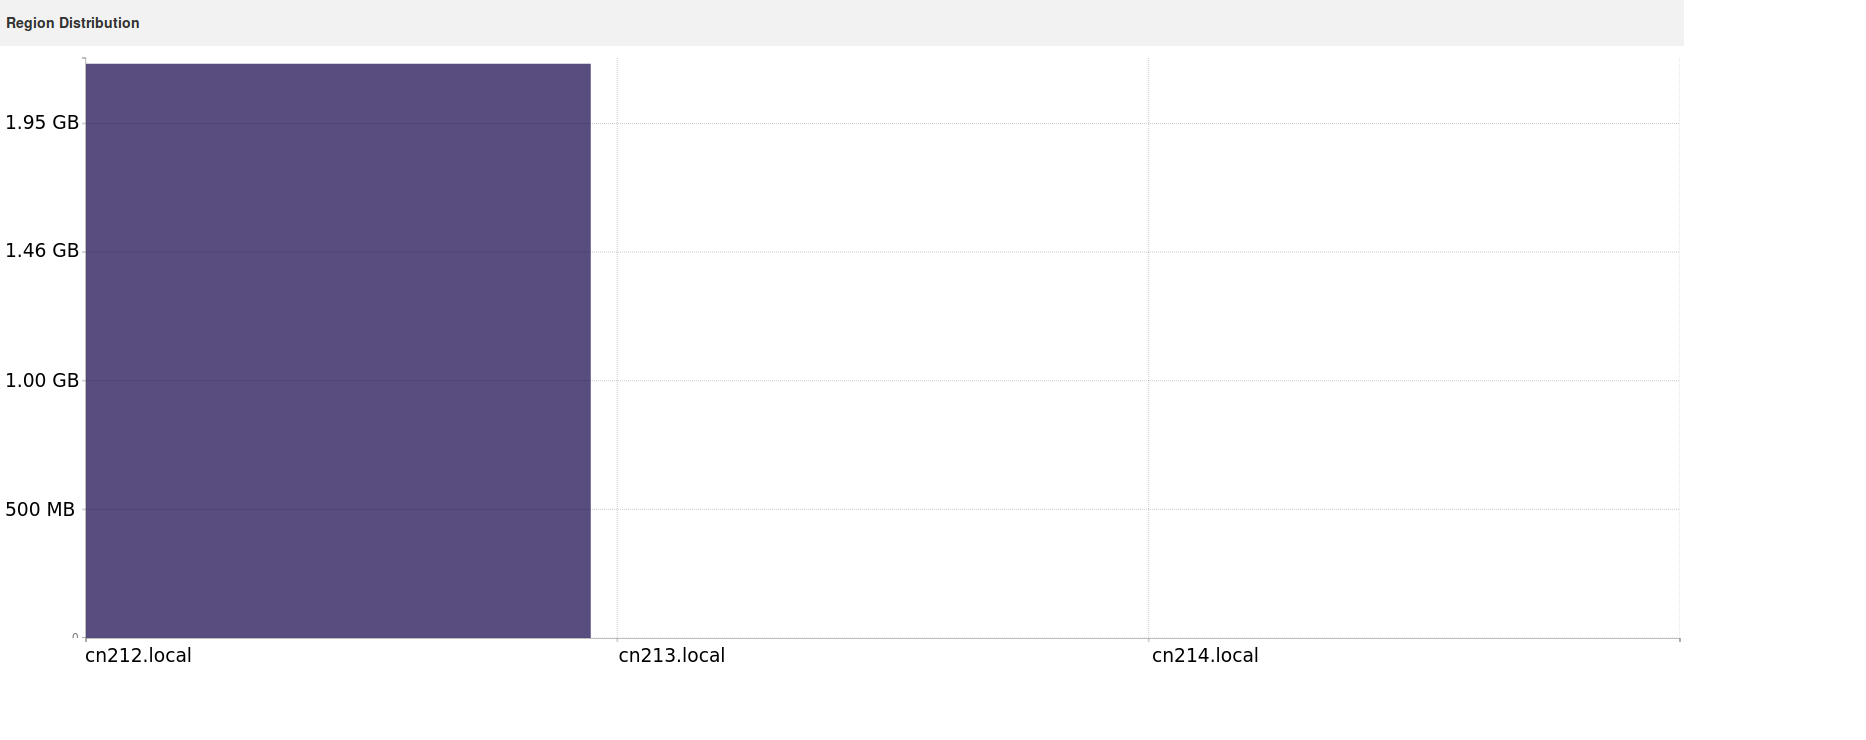
\includegraphics[width=1.2\textwidth,height=0.41\textheight]{./images/1regionserveractive1.png}
\caption{HBase one active Region Server.} \label{fig:1regionserveractive}
\end{figure}


\item{Region Server handler count:}
\par
Region server keeps a number of running threads to answer incoming requests to user tables. To prevent region server running out of memory, this property is set to 10 by default which is a very low number unless you are using large write buffers with a really high number of concurrent clients. In our case, that our payload per request is low, increasing this number to handle more requests from the client would be beneficial as it will mean more accepted concurrent write requests. On the other hand, setting it to a higher number will consume more Region server's memory, but our cluster has enough to handle this peak. So in order to leverage it, we need not just to change \textit{hbase.regionserver.handler.count} parameter which affects the server-side, but also to make the client to work concurrently by using threads.

\bigskip

\centerline{\textit{hbase.regionserver.handler.count = 10}}
\bigskip
\item Compressed data:
\par
In Hbase, it is well-known that using some form of compression for storing data may lead to an increase in IO performance, and thus in an increase in the overall performance \cite{raichand2013short} \cite{cheng2013key} \cite{aiyer2012storage} \cite{ApacheHBaseCompression}. But at this point, we are not using any sort of data compression yet. We should exploit it to reduce the number of bytes written/to read from HDFS, to save disk usage and to improve the efficiency of network bandwidth. On the other hand, if we enable it, we will need to un/compress data so we will need some extra CPU cycles. It is simply trading IO load for CPU load.

%\fixme{Talk in another approach about the three codecs with some graphs? or just here: I will use Snappy because balbalbala?  %http://blog.erdemagaoglu.com/post/4605524309/lzo-vs-snappy-vs-lzf-vs-zlib-a-comparison-of }
 \bigskip

\item setAutoFlush:
\par
HBase client API provides a built-in \textit{Write Buffer} which allows to cache a group of \textit{Put/Delete} objects on the client side, and flushes these objects to the Region Servers in a batch so that they are sent within one RPC call to the servers, instead of sending \textit{Puts} one at a time like by default. Using it, all requested changes will wind up in the same Write Buffer and will not be sent until the Write Buffer is filled. The chief advantage of using it is the reduction in the amount of necessary RPC connections to transfer data from the client to the sever and back. In our application, which needs to store thousands of values per second, less RPC calls will mean less round-trip times (RTTs) to happen. Figure 5.1 provides the architecture of the Client Write Buffer \footnote{This figure is obtained from HBase: The Definitive Guide}.

\bigskip
\begin{figure}[htb]
\centering
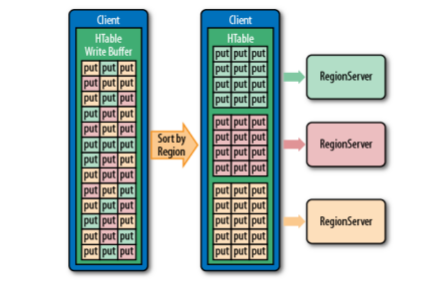
\includegraphics[width=0.7\textwidth,height=0.25\textheight]{./images/putsRegionServer.png}
\caption{HBase built-in Write Buffer.} \label{fig:putsRegionServer}
\end{figure}

To take advantage of this feature, we must \textit{setAutoFlush} to false, instead of true by default.

\bigskip
\item Write Ahead Log:
\par
We have already explained the HBase architecture and its Write Path, where WAL plays and is on by default. Turning WAL off indicates that Region server will not write \textit{Put} objects into the WAL, only into the MemStore and thus, increasing throughput on Puts. In return, if there is a Region server failure there will be data loss.

\end{enumerate}


All of these drawbacks will be kept in mind as the base to improve our subsequent solutions.

\subsubsection{Second version: An HBase client without AutoFlush}

This is a minor modification to the first approach. Disabling setAutoFlush reveals a slight improvement:
\par
\centerline{Results.}




\subsection{Second approach: A multithread HBase client}

In this proposal we have improved our first HBase client application by adding support to Java threads. The idea behind it is very simple: instead of reading and parsing XML video files one at a time, we create now N Java threads and each of them reads and parses one file concurrently. There is no limitation with our hardware since our nodes have twelve cores each one and they can run multiple threads. The issue resides in the HBase API because the \textit{HTable} class we are using is not thread-safe, that is, the local write buffer is not guarded against concurrent modifications. To dodge it, we should use one instance of HTable for each thread we are running in our client application, and that is exactly what \textit{HTablePool} class allows us to do: namely to pool client API instances to the HBase cluster.
\par
\textit{SetAutoFlush} is turned off for each HTable within the pool as we gain performance with it (this feature is not available in HBase 0.92.X series but now it is possible thanks to the HBASE-5728 patch \cite{HBase5728}). 
\par
 In our experiments we have tried from 2 to 50 HTable instances / threads with different numbers of RPC listener threads turning out the following results:


\begin{figure}[htb]
\centering
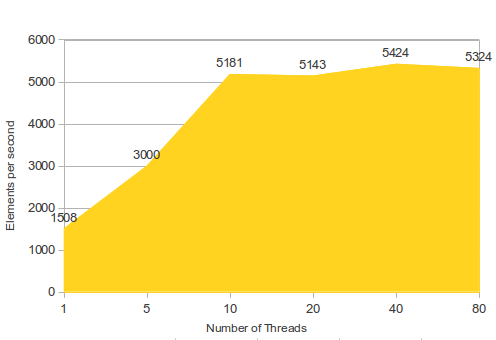
\includegraphics[width=1\textwidth]{./images/threadsworking.png}
\caption{Elements per second processed.} \label{fig:threadsworking}
\end{figure}




*Hint:Logs do not reveal issues with Memstores and related parameters yet.

\bigskip

As we proceed before, it is time to discuss the drawbacks we discovered here:
\begin{enumerate}
\item WAL is still turned on. We have not disabled it because we do not want data loss in case of hardware or software failures. In the HBase Client API approaches, we place integrity before speed.

\item Still facing the problem of regions and Load Balancer.

\item Data continues uncompressed.

\item Above all drawbacks and most important point: thread job is bounded by disk seeks. Currently, XML files are stored into the underlying file system ext4 and not into a distributed file system such as Hadoop HDFS.
\end{enumerate}


\subsection{Third approach: Using MapReduce algorithm}


Up to this point, we use Hadoop HDFS as the distributed file system for our HBase cluster, but we have not taken advantage of the processing framework Hadoop provides, which is MapReduce and its tight integration with HDFS and these two with HBase.
\par
Hbase includes several methods to support loading data into HBase. The two most straightforward solutions are either to use the \textit{TableOutputFormat} class from a MapReduce job to write data into an HBase table or to use the default HBase client APIs. If there is not too much data to transfer, using the latter one is the best and also the simplest option, but when data is voluminous, using \textit{TableOutputFormat} MapReduce job to load data makes more sense. Even more, instead of using the last one, is more efficient to generate the internal HBase format files (HFiles) within our MapReduce job and then load the generated files into our HBase cluster. This feature is namely \textbf{Bulk Load} and it uses less CPU and network resources than simply using the \textit{TableOutputFormat} API or any other HBase client APIs \cite{ApacheHBaseBulkLoad}. Therefore, our third approach is based on \textbf{Bulk Loading}. In the following lines we explain what steps we took to get this third solution up and which were the issues we coped with.

\subsubsection{Building the solution}

First of all is to get to know how MapReduce really works and what drawbacks it has. If we want to leverage the power of the MapReduce framework at its maximum, we must place all our XML files into the Hadoop HDFS file system, because is how MapReduce achieves its best performance. The place where MapReduce really shines is if data gets stored on several different nodes (a distributed file system) and its mappers can access different partitioned data on different nodes in parallel. But, before copying the data from the local file system to HDFS, we have to deal with Hadoop HDFS and MapReduce small files problem.

\paragraph{The Small Files problem \cite{liu2009implementing}:} In terms of Hadoop HDFS, a small file is one which is smaller than the HDFS block size (in our case, 64MB). The problem with them is that HDFS is not designed to handle a lot of files due to every file, directory and block in this distributed file system is represented as an objects in the NameNode's memory, so having lots of files would use too much memory. Thus, HDFS is not geared up to efficiently accessing small files, but for streaming access of large files. 
\par
MapReduce also suffers the same issue due to mappers usually process a block of input at a time. If there are lots of small files, there will be a lot of more mappers, with their corresponding bookkeeping overhead. To overcome this pitfall and to be able to exploit the real power of MapReduce we have rewritten all the XML files together into a big single \textit{SequenceFile} (a Hadoop-specific archive format) \cite{ApacheHadoopSequenceFile}, in which the name of each file is the key and its file contents is the value. 
\par
\textit{SequenceFiles} are splittable. MapReduce can cut them into chunks and interact with each one autonomously. They support compression and splitting as well, which is another advantage to keep in mind since MapReduce jobs performance is increased when working with splittable files (they can be processed in parallel by many mappers)  \cite{SmallFiles}. Figure 4.2 samples the SequenceFile file layout \footnote{Figure extracted from Cloudera Small Files Problem article.}

\begin{figure}[htb]
\centering
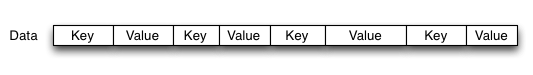
\includegraphics[width=0.8\textwidth]{./images/sequencefile.png}
\caption{SequenceFile File Layout.} \label{fig:sequencefile}
\end{figure}


To load all the XML files into a big single \textit{SequenceFile} we have created an application for managing SequenceFiles. It allows us to create a SequenceFile with a key, which will be the name of the corresponding XML file, as a \textit{Hadoop Text} type and the value, which will be the file contents, as a \textit{Hadoop Text} type as well.
\par
Up to this point, we have managed to get our data ready to efficiently feed our MapReduce job. Now  it is time to expose how our MapReduce client looks like and what results it gives out.

\bigskip

%\fixme{what about some MapReduce code here ?.}

%\bigskip

In our MapReduce Java code we first create a Job instance and then we set different parameters to it, such as the InputFormatClass, OutputFormatClass, MapOutputKeyClass, MapOutputValueClasse, etc. One of these parameters is the mapper class. Our map tasks receive \textit{Text} keys, and \textit{Text} values one at a time. The key is the name of a XML file and the value is its file contents. Each spawned map task parses the XML content, creates the corresponding Put objects, adds parsed data to the Put object and finally, unlike previous approaches where the Put objects were written directly to the HBase table, the map task passes fully completed Put objects to the reducers by calling \textit{context.write()} method.
\par
Along with the Bulk Load feature,we use \textit{configureIncrementalLoad}, a method provided by HBase to auto configure the reduce phase. It establishes \textit{PutSortReducer} class as the reducer method, because it sorts columns of a row before writing them out, ensuring the total order at column level HBase needs. In addition, it sets \textit{TotalOrderPartitioner} as the partitioner class to ensure total order partitioning at a row level too. As we wrote before, Bulk Load feature generates HBase internal data files from a MapReduce job using \textit{HFileOutputFormat}. It must be configured in such a way that each output HFile is matched to a single region and that is why this kind of MapReduce jobs use \textit{TotalOrderPartitioner} class: to partition the map output into disjoint ranges of the key space, which correspond to the key ranges of the current regions in the table. The number of reducer tasks is set according to the number of regions in the table, that in our case it is still one.

\subsubsection{Third approach second version: Compression}

Finally, after some approaches, we try out compression. For this solution we have used the final code we got from the previous approach; the MapReduce client version. Compression has been enabled in both mappers output and reducers final outputs (HFiles) by setting these parameters to the job:

\begin{table}[htbp]

\begin{tabular}{|l|}
\hline
job.getConfiguration().setBoolean("mapred.compress.map.output", true); \\ \hline
job.getConfiguration().setClass("mapred.map.output.compression.codec", \\ \hline
org.apache.hadoop.io.compress.XXXCodec.class, \\ \hline
org.apache.hadoop.io.compress.CompressionCodec.class); \\ \hline
job.getConfiguration().set("hfile.compression", \\ \hline
org.apache.hadoop.hbase.io.hfile.Compression.Algorithm.XXX.getName()); \\ \hline
\end{tabular}
\label{}
\caption{MapReduce compression parameters}
\end{table}

One extra benefit on using compression in the reducer side within the Bulk Load feature is that the final outputs we will get from it will be the internal HBase files which will constitute our database (HFiles) and they will be already compressed. All of this will give us an HBase database with all its data already compressed.
\par
As we justified in the first approach, using compression is beneficial for us. It reduces the size of our final data and the amount of data exchanged between mappers and reducers by losing just some CPU cycles. Using compression makes even more sense in MapReduce jobs since they are nearly always IO-bound processes and not CPU-bound.
\bigskip
\par
Hadoop allows to use a variety of compression algorithms, although the more adopted ones are DEFLATE, GZip \cite{GZip}, LZO \cite{oberhumer2005lzo} and Snappy \cite{Snappy} \footnote{Hint = Snappy is nonspittable out of Hadoop, but it can be used for block compression within lot of Hadoop file formats, such as HBase tables, Avro Data Files and SequenceFiles.}. Table 5.4 shows a brief comparison between this compression codecs.
\begin{table}[htbp]

\begin{tabular}{|l|l|l|l|l|}
\hline
Compression format  & Tool  & Algorithm File  & Extension  & Splittable \\ \hline
gzip &  gzip  & DEFLATE  & .gz &  No \\ \hline
LZO &  lzop &  LZO  & .lzo &  Yes if indexed \\ \hline
Snappy  & N/A  & Snappy  & .snappy  & No \\ \hline
\end{tabular}
\label{}
\caption{HBase Compression formats}
\end{table}


All compression algorithms exhibit a space/time trade-off. Gzip is a general purpose compressor, and sits in the middle of the space/time trade-off. LZO and Snappy are optimized for speed, which means less effective compression but more faster than its competitors. Snappy is also faster than LZO for decompression \cite{CompressionHadoop}. Figure 5.6 depicts the results.


\begin{figure}[htb]
\centering
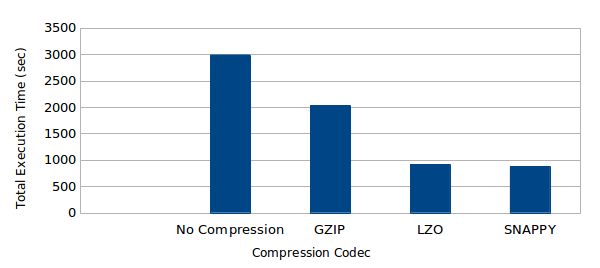
\includegraphics[width=1\textwidth]{./images/codecs1.png}
\caption{Total time to Import the dataset with different compression codecs.} \label{fig:codecs}
\end{figure}


Although LZO is close to Snappy, this later gives out the best speed up. GZIP is far slower than its competitors.

Hence, analyzing our results and reading other studies about compression codecs conducted in HBase \cite{CompressionComparison}, we have chosen Snappy as our compression format for both intermediate files of the map phase and final MapReduce output (HFiles) for the next rounds of studies.




\subsubsection{Third approach third version: Pre-creating regions}
Here is where we address one of our older issues already discovered in the first approach: The method admin.createTable() creates a table with only one region. Now, that we are using Bulk Load MapReduce feature, we can see how this issue continues here just by glancing at Hadoop logs:

\bigskip

INFO mapreduce.HFileOutputFormat: \textbf{Looking up current regions} for table org.apache.hadoop.hbase.client.HTable@40be76c7
\par
INFO mapreduce.HFileOutputFormat: \textbf{Configuring 1 reduce partitions to match current region count}

\bigskip

The \textit{HFileOutputFormat.configureIncrementalLoad} method looks up the current regions for our table and finds one, that is why it configures  only one reduce partition (one reduce partition per region). Only one reducer task will be spawned, while the rest of the nodes will stay idle.




\begin{figure}[htb]
\centering
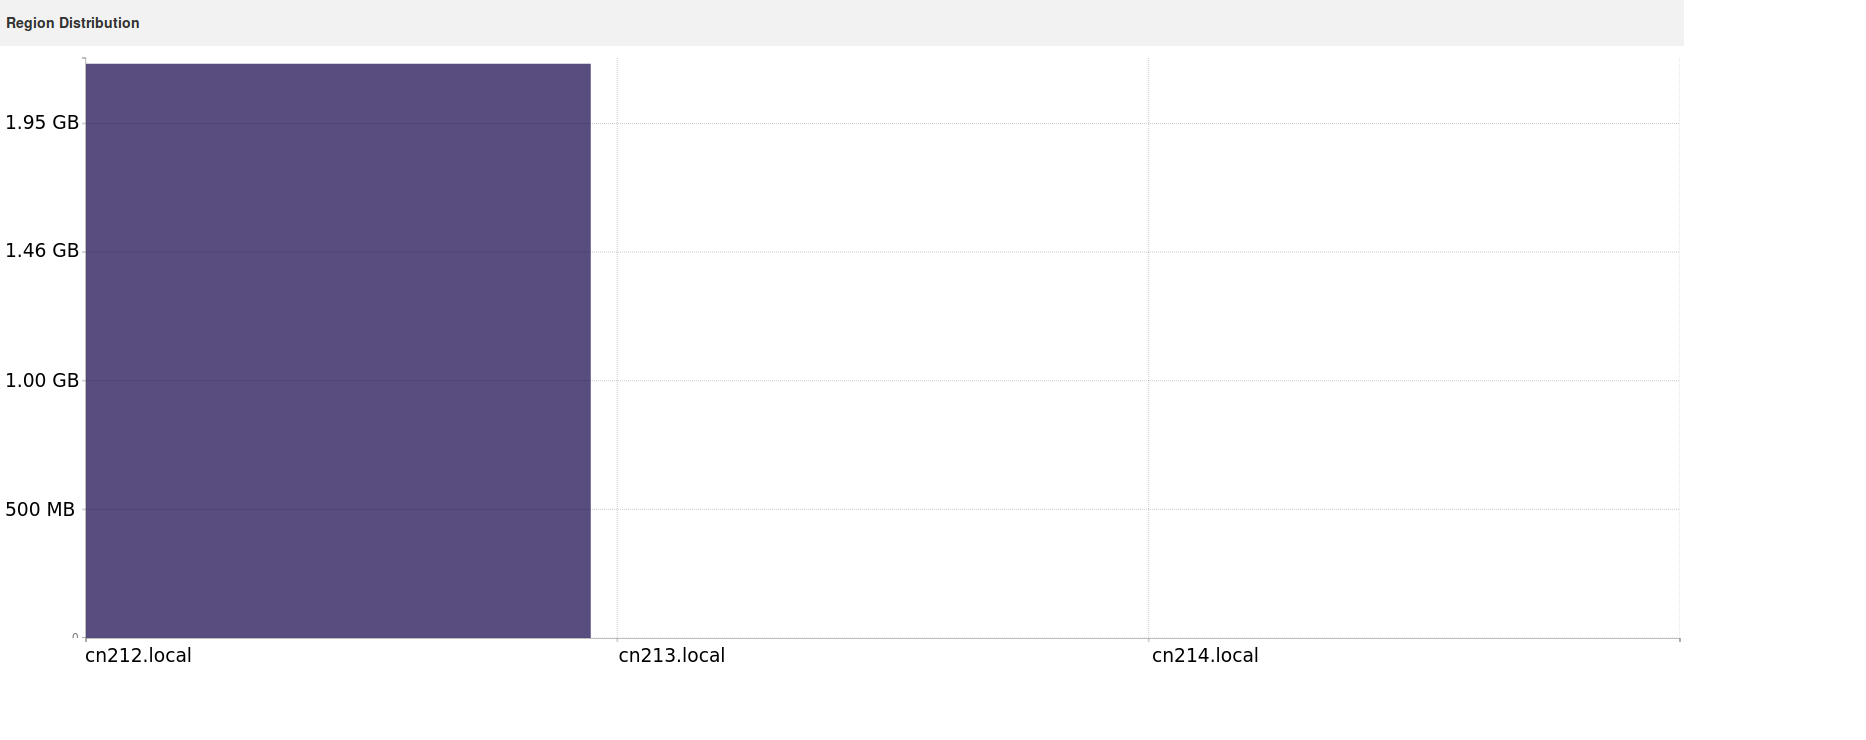
\includegraphics[width=1\textwidth,height=0.34\textheight]{./images/1regionserveractive1.png}
\caption{HBase one single Region Server.} \label{fig:oneRegion}
\end{figure}



Looking at the figure 5.7, we can see how data ends up within a single region in one Region Server. If we create an HBase table with only one region, all clients will only be able to write out to the same region until it gets split and distributed across our cluster. The solution is to pre-create a table with the desired number of empty regions; \textit{Admin.createTable(table, startKey, endKey, numberOfRegions)} method allows us to do exactly what we want. It creates a table with \textit{numberOfRegions} regions and as first split the passed \textit{startKey} and as last split the \textit{endKey}. We have configured it to pre-create 24 Regions in order to match the number of total reduce slots our cluster allows and thereby to complete the job spawning only one single wave of reducers. Figure 5.8 reveals a slight improvement performance in the needed time to import the dataset into HBase.


\begin{figure}[htb]
\centering
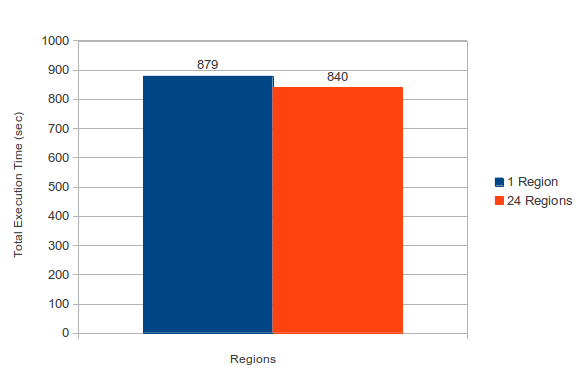
\includegraphics[width=1\textwidth]{./images/1-24regions1.png}
\caption{Execution time to import the dataset with different number of pre-created regions.} \label{fig:regions}
\end{figure}

Despite the performance enhancement, a closer look at the taskTracker logs reveals some issues. Albeit all nodes are working now, some nodes are working harder than others. The graph 5.9 depicts the region distribution across the four region servers. Node cn212 stores the 72.22\% of the total data, making an uneven distribution of it across the Region Servers. Next graph, 5.10, shows the sizes of the 24 regions created. As before, data has been uneven distributed: Region 1 stores the 70\% of the dataset.




\begin{figure}[htb]
\centering
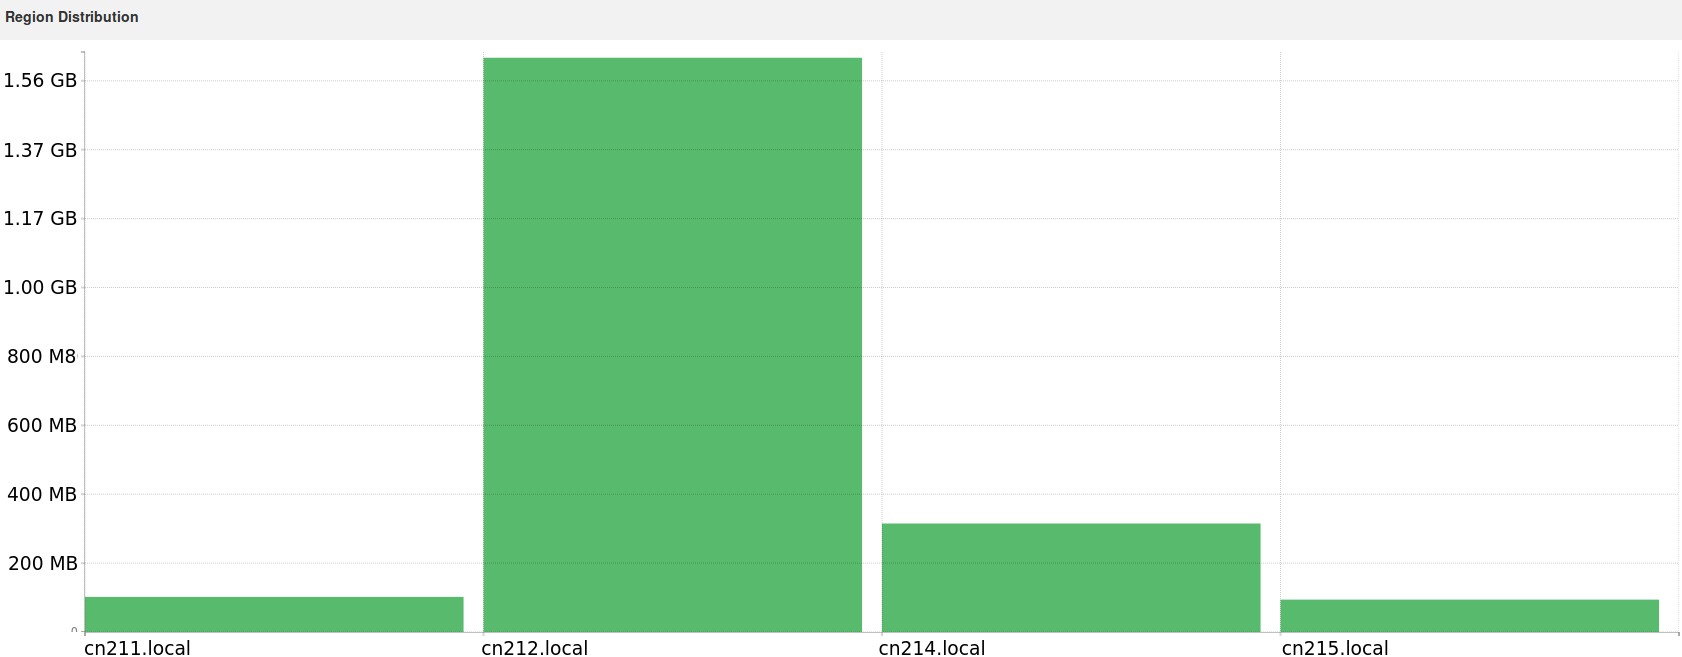
\includegraphics[width=1\textwidth,height=0.31\textheight]{./images/regiondistribution1.png}
\caption{Uneven region server distribution.} \label{fig:regionDistribution}
\end{figure}



\begin{figure}[htb]
\centering
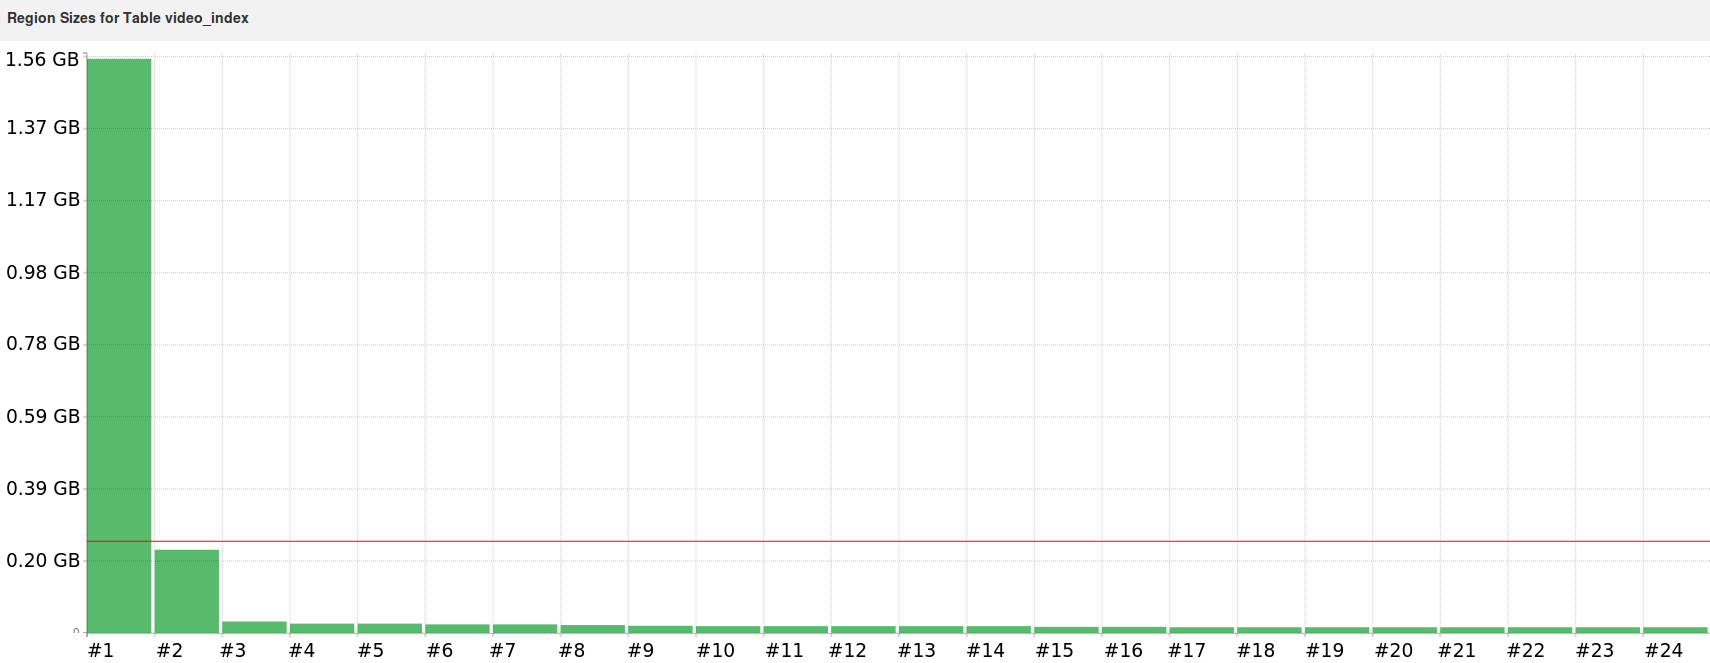
\includegraphics[width=1\textwidth,height=0.31\textheight]{./images/24regions1.png}
\caption{24 uneven regions.} \label{fig:24evenRegions}
\end{figure}

TaskTracker logs uncover what is the problem: some reducers are working with more than 10 times the amount of records others are dealing with, which translates to different reducer execution times. While some finish within less than a dozen of seconds, others takes more than 5 minutes. 
\par
This happens because data's keyspace is not evenly distributed. \textit{Admin.createTable(table, startKey, endKey, numberOfRegions)} flaw is that it uses \textit{Bytes.split} as the split strategy and it does not work efficiently with uneven data. All the regions are accessible in the keyspace, but since our keyspace is not evenly distributed, some reducers/regions does not receive almost any data, while others collects nearly all data.



\subsection{Fourth approach:Skew data}

What we have experienced in the last approach is called \textit{Skew} in a MapReduce environment. Skew refers to a significant load imbalance and its causes have been widely studied \cite{ananthanarayanan2010reining} \cite{dean2008mapreduce} \cite{walton1991taxonomy}. Skew can appear due to computational load imbalance, characteristics of the user-defined operations or of the specific dataset or by hardware malfunction among others reasons. Skew from either cause is undesirable because it leads to longer job execution times and throttles cluster throughput. The original MapReduce paper \cite{dean2008mapreduce} tackles this problem using speculative execution. Albeit this works well, it is not the best solution since it means repeating work already done.
\par
Balazinska \textit{et al.} identified a specific type of skew, referred to as \textit{Data Skew} \cite{kwon2013managing}: It affects both keys and values in either mappers or reducers. They state that data skew occurs more often for the reducers because mappers mostly take the same-size blocks of input data. There are two sub-types of this skew: one caused by uneven data allocation; the number of key values for one task is much larger than the number of keys in the other partitions to cause an imbalance. A second one caused by uneven processing times; one task processes larger number of values than the other tasks. 
\par
According to our Hadoop cluster logs, data skew happens in the reducer phase because almost all mappers take the same time to complete their tasks but not the reducers. A deeper insight into logs reveals some reducers taking significantly larger number of keys than the other reducers. This is what is causing the imbalance situation and is referred to as \textit{Reduce phase: Partitioning skew} \cite{kwon2012skewtune}.
\par
In our MapReduce job, map tasks outputs are distributed among reduce tasks via \textit{TotalOrderPartitioner}, which partitions the map output into ranges of the keyspace, which correspond to the region boundaries of our HBase table created by the \textit{Bytes.split} method. This is not adequate for our data because it is not evenly distributed. There are lot of duplicated keys and a big part of them are really similar, ending up in the same region.
\par
To cope with this problem, we have to somehow find a good partitioning function that ensures total ordering, like TotalOrderPartitioner does, and splits the data into equal partitions as well. Hadoop provides a partitioning function called \textit{InputSampler}, which sample the input at random or what user choose to estimate what is the best way to partition. But since it samples the map input data, it does not fit our needs. What we need to sample is the map output, which will be the keys of our table. That is why we have developed a lightweight MapReduce Java-based tool which samples map output keys and gives us a file describing the best partition for our dataset. Subsequently, this file can be used in combination with \textit{TotalOrderPartitioner} to know which key/value pairs to send to which reducers, or it can be used in combination with \textit{admin.createTable(table, splitPoints)} method to create a table with the best split points for regions in MapReduce-HBase environments. This file will be able to evenly span the key space creating an even distribution of records across the reducers and to create regions with almost the same size, therefore having a well apportioned HBase cluster.
\par
Our sampling tool uses a wrapper input format that makes a record reader which passes few key/value pairs to the mapper. The rate at which key/value pairs are passed to the mapper can be modified according to user needs. In order to obtain a significant sampling of the entire data, adjust it to ten has been tested to be valid enough for us. Ten gives a good speed/significant-sample ratio. The mappers of the sampling job emit only keys, while the values are always null. In order to reduce the total amount of generated data, the XML files are not completely parsed, it just needs the ids of each element. Finally, our tool also overwrites the input format with a sampling reducer that emits the exact number of samples needed for the creation of the regions of the HBase table. 

\bigskip

Next table shows how fast the sampling tool gets his job done: 

\begin{table}[htbp]
\begin{center}
\begin{tabular}{|l|l|}
\hline
Sampling input dataset & 83 sec \\ \hline
\end{tabular}
\caption{Sampling time result.}
\end{center}
\label{Results}
\end{table}

We have modified the old MapReduce job to accept the text file created by the sampling MapReduce tool and to create the HTable with the new and correct splits points.
\par
The maximum number of reduce tasks that will be run simultaneously by a task tracker is set to 6 (\textit{mapred.tasktracker.reduce.tasks.maximum}). Hence we create 24 regions in our table. 4 regions per node (6 simultaneous reducer tasks {*} 4 nodes = 24). Therefore, the job will only need one single wave of reducers to complete it. On the other hand, each map tasks will read off one DFS block, so multiple map waves will be used getting hide shuffle latency.


\begin{figure}[htb]
\centering
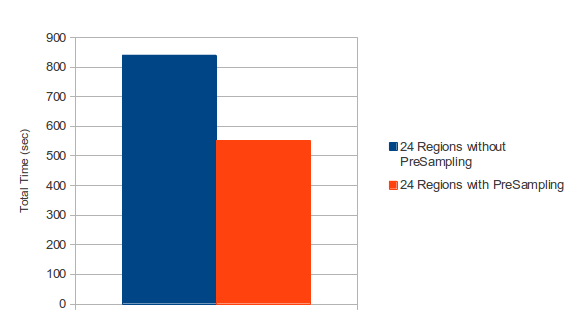
\includegraphics[width=1\textwidth]{./images/24regionsChartSampling.png}
\caption{Total time to import data with and without using our Sampling Tool.} \label{fig:regionDistribution3}
\end{figure}

Figure 5.11 shows the outcome of our tests. Using our Sampling Tool we have reduced the total execution time to import data to only 552 seconds, which is 34.29\% faster than our previous results with pre-created Regions. Figure 5.12 depicts the region distribution obtained using the Sampling Tool. Now, data is much even distributed along the four Region Servers. Digging into logs reveals more uniform reducers' execution time as well.


\begin{figure}[htb]
\centering
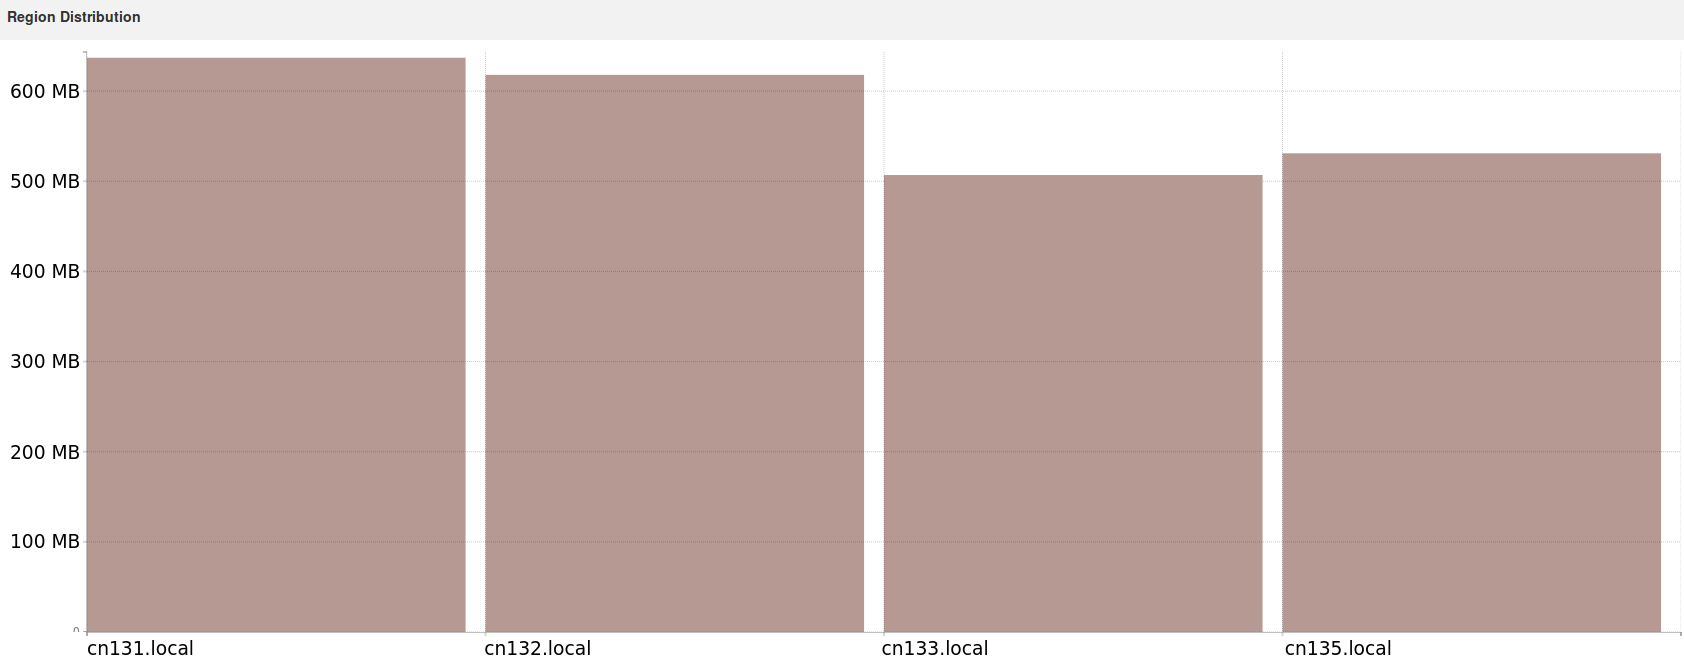
\includegraphics[width=1\textwidth,height=0.31\textheight]{./images/usingSampling1.png}
\caption{Region distribution using our sampling tool.} \label{fig:regionDistribution2}
\end{figure}


\fixme{Give thanks to Chase Bradford for the idea.}


\section{Performance Tunning Hadoop}

At this point, we have reached the best possible importing performance level in our HBase cluster without going to deep into Hadoop parameters, so now we can start to fine tuning these configuration details in order to maximize the performance of our Hadoop workload. This tuning has been performed by taking the last approach as our baseline and following well-known studies about Hadoop performance tuning \cite{babu2010towards} \cite{heger2013hadoop}. In the following lines, we explain which parameters we have hacked and why:

\begin{itemize}
\item \textbf{HDFS block size}: In our Hadoop cluster, each mapper receives an input split whose size is determined by \textit{dfs.blocksize} (by default, 64MB). If we increase it, the number of spawned mappers will decrease and less overhead will be created as there will be less map output splits to merge and less map tasks to run. On the other hand, the execution time taken by each mapper will increase. 
\par
Figure 5.12 shows the performance with different HDFS block sizes. Our optimal size comes out to be 128MB.

\begin{figure}[htb]
\centering
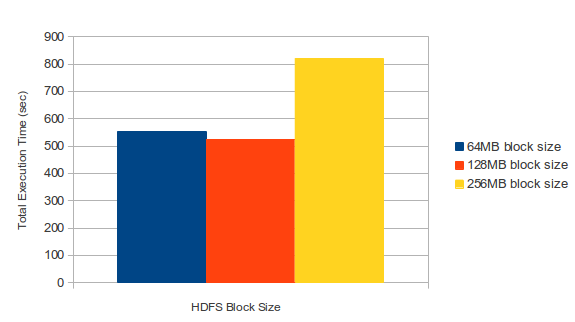
\includegraphics[width=1\textwidth]{./images/HDFSBlockSize.png}
\caption{HDFS block size setting.} \label{fig:HDFSBlockSize}
\end{figure}


%\fixme{http://developer.amd.com.php53-23.ord1-1.websitetestlink.com/wordpress/media/2012/10/Hadoop\_Tuning\_Guide-Version5.pdf}


\item \textbf{Spilled records}: While mappers are running, the generated intermediate output of map tasks is hold in buffers. Mappers have assigned a portion of memory of the map JVM heap in which they store their results, but if it gets completely filled up, its contents are spilled to disk. If this situation happens multiple times, it leads to additional overhead, which means more time to complete the phase. 
\par
If we study our logs, we can see that the total \textit{Map output records} is much lower than the \textit{Spilled records}, which indicates that we are not setting an appropriate size for the buffers, they are being spilled to disk many times. To avoid this, we hack the value of the parameter \textit{io.sort.mb}, which is by default 100MB to be big enough to hold all the records. By doing some calculations, setting it to 1280 MB fits our needs. Less records are spilled to disk and only the compulsory and final spill is done once the mapper is completed.
\par
If the input size of each mapper is 64MB:
\bigskip

\centerline{Our records have in average 3202.81 bytes/record}
\centerline{so if the block size is 64MB we have 20953.12 records/input}
\centerline{Every spilled record takes 16 bytes of metadata in buffer, so 20953.12 * 16 = 0.32MB}
\centerline{io.sort.mb = 64MB data + 0.32MB metadata = \textbf{65MB} needed.}

\bigskip

If the input size of each mapper is 256MB:

\bigskip
\centerline{Our records have 3202.81 bytes/record in average}
\centerline{so if the block size is 128MB we have 41906.24 records/input}      
\centerline{Every spilled record takes 16 bytes of metadata in buffer, so 41906.24 * 16 = 0.64MB}
\centerline{io.sort.mb = 128MB data + 0.64MB metadata = \textbf{128.64MB} needed.}
\bigskip
\par
We are still far away from the spill threshold setting. 

\bigskip

Same happens with the reducers, before applying the reduce function they need to copy, merge and sort the map outputs, so they start copying records from mappers and storing them in a buffer until a threshold is reached and then, these records are spilled to disk. The size of this buffer is governed by \textit{mapred.job.shuffle.input.buffer.percent} parameter and its default value is 66\% of the Reduce JVM heap space. The ideal scenario would be one where this buffer would be big enough to hold all map output records, but since it is a too high size or sometimes is even impossible to reach, increasing this percent to a higher number will be enough for our purposes. Finally, after running several tests, we saw performance improvements by increasing this parameter to 90\%.
\par 
Another related parameter is \textit{mapred.job.reduce.input.buffer.percent}, set by default to 0\%. It imposes the size of the Reduce JVM heap that is allocated to the final reduce function. Since our reduce function is not memory-bound, we can use a JVM heap percent to retain some records and thus reduce the number of IO operations. Consequently, we set it to 80\%.


\begin{figure}[htb]
\centering
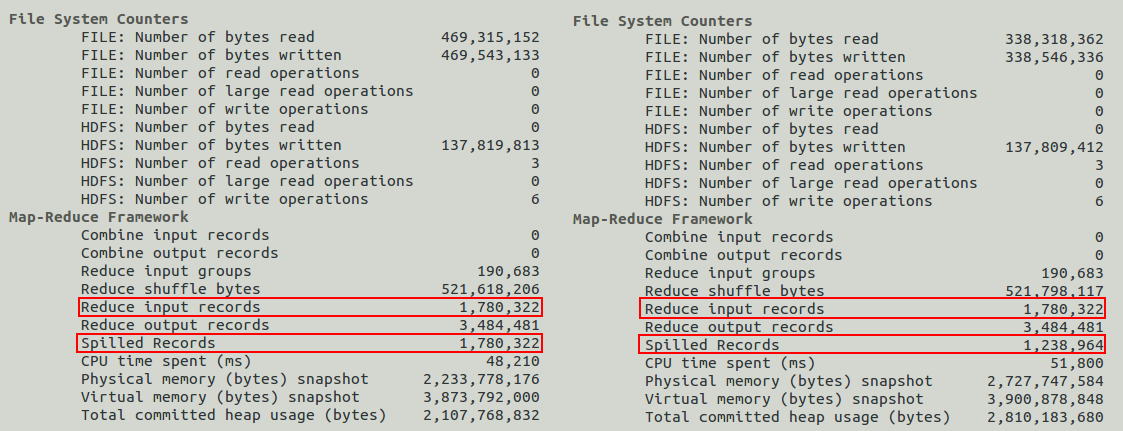
\includegraphics[width=1\textwidth]{./images/spilledReducerRecords.png}
\caption{Spilled records in reducer side.} \label{fig:spilledReducerRecords}
\end{figure}

The left side of the figure 5.14 reveals that all the reduce input records (1780322 records) were spilled to disk within a given reducer task, while the right side of the figure shows that only 1238964 of a total of 1780322 records were spilled to disk. For the left side, the default settings described above where used, while for the right side, we hacked them whit the ones stated before.


\end{itemize}









%SUBE EL MALDITO IO.SORT.MB Y FS.INMEMORYSIZE.MB

%ANYADIR CITA DE LA BIBLIA DE HADOOP, ese libro aunque sea mapreduce compression chapter.

%Maps 
%- Usually as many as the number of HDFS blocks being 
%processed, this is the default 

%Reduces 
%- Unless the amount of data being processed is small 
%0.95\*num\_nodes\*mapred.tasktracker.reduce.tasks.maximum

%The number of reducers is best set to be the number of reduce slots in the cluster (minus a few to allow for failures). This allows the reducers to complete in a single wave.

%So long as each task runs for at least 30-40 seconds, increase the number of mapper tasks to some multiple of the number of mapper slots in the cluster. If you have 100 map slots in your cluster, try to avoid having a job with 101 mappers - the first 100 will finish at the same time, and then the 101st will have to run alone before the reducers can run. This is more important on small clusters and small jobs.

%-DECIR QUE EN ESTE APPROACH EL WAL ESTA DESACTIVADO AL USAR BULK LOAD POR DEFECTO.

%ANYADIR A APPROACH 1 Y 2 QUE EL METODO LLAMADO Y QUE HACE ES EL VIDEO.PUT() COMO EN ESTE APPROACH

%HABLAR SOBRE LA BIBLIOTECA DE PARSEO!

%Hablar de Zipfian





